\section{Subject Interaction}

\subsection{Subject, Messages, and their Interaction}
\label{sec: Subject}


\begin{figure*}[htbp]
	\centering
	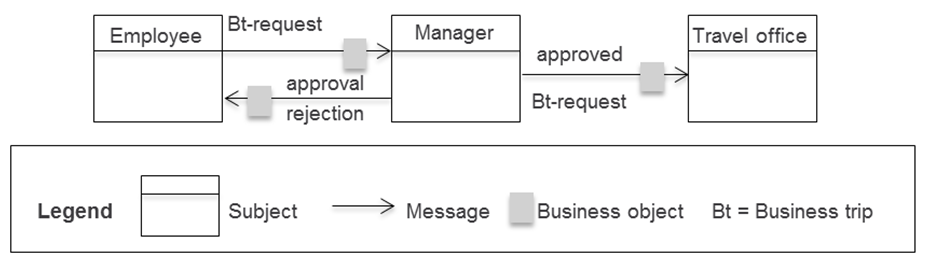
\includegraphics[width=14cm]{Figures/Ontology/SubjectInteraction/Beispiel-Subject-Interaction.png}
	\caption[Subject interaction diagram]{Subject interaction diagram for the process 'business trip application'}
	\label{fig:beispiel-SubjectInteraction}
\end{figure*}

As already detailed previously, subjects defined in a Subject Interaction Diagram, represent an active entity in a process context. This consistency should also be reflected in its name or lable and differ it from the passive Objects in the SID or the Activities in the SBD. Note that a specification of a subject does not say anything about the technology used to execute its corresponding behavior. 

Subjects communicate with each other by exchanging \textbf{Messages}. A subject sends messages to other subjects, receives messages from other subjects, and executes internal actions. All these activities are done in logical order which is defined in a subject's behavior specification (its SBD).

In general, there are two principle types of subjects:

\begin{itemize}
	\item Fully specified subjects
	\item Interface subjects 
\end{itemize}

Both come in the variant of:

\begin{itemize}
    \item Multi-subjects
	\item Single subjects
\end{itemize}

\subsubsection{Fully Specified Subjects}

The \textbf{Fully Specified Subject} is the standard subject type. Fully specified subjects consist of the following components:

\begin{itemize}
    \item \textbf{Subject Behavior Diagram (SBD)} --- to specify its behavior in the modeled process context. The behavior of each subject describes in which logical order it sends messages, expects (receives) messages, and performs internal functions. Messages transport data from the sending to the receiving subject and internal functions operate on internal data of a subject. 
	\item \textbf{Data Definition} --- Each subject is assumed to have a private data storage that contains e.g. business objects relevant in a modeled process context. Examples for contained data are business trip requests, purchase orders, packing lists, invoices, etc. Business objects are composed of data structures. Their components can be simple data elements of a certain type (e.g., string or number) or other complex data structures themselves - the exact means to specify the structure and types of the internal data store of a subject are identical to the mans to specify the payload of massages as described later.
	\item Outgoing \textbf{Message Exchanges} (Sent messages) --- Messages which a subject sends to other subjects. Each message has a name and may transport some data objects as a payload.
	\item Incoming \textbf{Message Exchanges} (Received messages) --- Messages received by a subject. The values of the payload objects are copied to business objects of the receiving subject.
	\item \textbf{Input Pool Restrictions and Handling Strageis} --- Modeling with PASS assumes that during execution of the process, messages sent to a subject are deposited in the \textbf{input pool} of the receiving subject. In principle the size of an input pool is not restricted. However modeling means 
	\item \textbf{Instantiation Restriction}  --- It may be limited how often a Subject may be instantiated or exist in a given process context and in relation to other subjects in the model (See also \textit{Multi-Subject})
\end{itemize}

Fully Specified Subjects are also called \textit{Internal Subjects} - as in being defined inside a given model - in contrast to \textit{Interfaces Subjects} that are also known as \textit{External Subjects}.

\subsubsection{Interface Subjects}

Interface subjects are used to model interfaces to other process systems. They neither have a behavior nor a data definitions in a given model, but they can be target or origin of Message Exchanges and may be restricted in their instantiating.

Interfaces subjects are used when the behavior of a subject is either unknown, if they are not of importance to a model, e.g., if they are too simplistic or modeling would require more effort than the benefit it would bring. Alternatively, the behavior of an interfaces subject is defined in a separate process system models which it may \textit{reference}. In that case their behavior is modeled \textit{externally} in another model - hence the older, alternative term of \textit{External Subject}.

Note: The "other" process models may represent a follow-up or a sub-processes. The exact meaning is up to the modeler, PASS does not explicitly defines on or the other.

\subsubsection{Multi-Subjects}

Both, Fully Specified as well as Interfaces subjects, may be defined to be Multi-Subjects. Multi-Subjects are subjects that may be instantiated multiple times within a process context, implying that there may be several actors executing copies of the same behavior.

This is useful if, e.g. in a process model several identical subjects exist that all do the same principle task in parallel to increase the throughput.  Another example would be a procurement process where bids from multiple suppliers are solicited and all suppliers in principle do the same thing - review the request and provide an offer. Once three offers have been received (from the supplier multi-subject), one is selected and actually ordered.

%If several communicating subjects in a process model are multi-subjects they can be combined to a multi-process.
%A process or sub-process is therefore executed simultaneously or sequentially multiple times during overall process execution. A set of type-identical, independently running processes or sub-processes is termed multi-process. The actual number of these independent sub-processes is determined at runtime.
 
%Multi-processes simplify process execution since a specific sequence of actions can be used by different processes. They are recommended for recurring structures and similar process flows. 

%An example of a multi-process can be illustrated as a variation of the current booking process. The travel agent should simultaneously solicit up to five bids before making a reservation. Once three offers have been received, one is selected and a room is booked. The process of obtaining offers from the hotels is identical for each hotel and is therefore modeled as a multi-process.

An interface subject (A) that is specified as a multi-subject may indicate that the whole corresponding process (sub-)system is instantiated multiple times (Multi-Process. Note that a fully specified subject (B) in another model, corresponding to a multi-interface-subject (A) in the first model, that  subject B is not necessarily a multi-subject itself if in the context of one instance of the whole (sub-)process there is only one instance of subject B. 

Note: While technically feasible to have only multi-subjects in a process model, it is assumed to be rarely useful as multiple subjects mostly make sense in the context where there are also single subjects. 1:1 (only single subjects) and 1:n scenarios are most common. n:m scenarios are rather complex and a modeler should be careful to consider if such a situation is really the best solution or if one or more simplified (1:m) models fulfil the same purpose.

Note: Technically, the Multi-Subject is the standard variant of a subject without any restrictions to number of time it may be instantiated in a given process context, in contrast to the \textit{Single Subject}.

\subsubsection{Single subjects}

Single subjects are all subjects, that are \textit{restricted} to be instantiated only once in the context of a given process model. They are used if for the execution of a subject a resource is required which is only available once.

Because many modelling tools have single subjects as the default modeling setting for subjects, single fully specified subjects can be considered as standard subjects.


\subsection{Messages and Payloads}

As stated, Subjects communicate with each other by exchanging \textbf{messages}. Messages have a name and a (data) \textbf{payload}. The name should express the meaning and content of a message informally. We recommend naming these messages in such a way that they can be immediately understood and also reflect the meaning of each particular message for the process\footnote{A good message name is akin to a good "subject"-description in an e-mail, giving the recipient a short summary of its content or meaning.}, but ideally also making clear that a message is a passive (data-) Object or piece of Information. In the sample 'business trip application', therefore, the messages are referred to as 'business trip request', 'rejection', and 'approval'.

In a model, message specifications define the principle information types or classes of data/information that can be send during execution. The default data payload of a message is empty - the creation of a message as well as its sending and reception is already an information that can be evaluated during execution. However, the payload specification can further define the information or data transported with the message. 

\begin{itemize}
    \item (formal) \textbf{Data Object Definitions}---If the message and its payload represent digital data to be transmitted within a IT system or similar means, that payload can be described with the means for classical data structure definitions. 
    \item \textbf{Physical Object Definitions}---If a PASS process model is not used as an instruction for an IT-System, but as a general description model for real life circumstances, message are not necessarily data objects but can rather also represent real elements, such as the transport of a physical good in an ordering process. Such an object can be described as the payload of a message but non-further specified natural language text or photos, etc..
\end{itemize}

If the described message payload is for the former, a digital data object, the messages serve as a container for the information transmitted. The payload may contain any number of data entries of two principle types:

\begin{itemize}
	\item Simple data types---Simple data types are string, integer, character. In the business trip application example, the message 'business trip request' can contain several simple data elements of type string (e.g., destination, the reason for traveling, etc.), and of type number or date (e.g., duration of the trip).
	\item Complex Data types/ (Business) Objects\footnote{Business Objects in their general form are physical and logical 'things' that are required to process business transactions. We consider complex data structures composed of elementary data types, or even other data structures, as logical \textit{business objects} in the context of a business processes model})---. For instance, the business object 'business trip request' could consist of the data structures 'data on applicants', 'travel data', and 'approval data' with each of these in turn containing multiple data elements.
\end{itemize}

There are many different means or technologies to specify passive data objects that allow to define, check and verify the structure of data or data objects --- the data type. Next to means in most object-oriented programming languages, often in the form classes, there are other languages such as e.g. XML schema\cite{w3d:xmlShema} for XML objects or also the RDF Schema \cite{rdf:rdfs}.

PASS in principle allows to use any of those to define the data type of payload elements. However, there is also a  build in definition means that allow to specify the existence of simple data field of payloads that are either of a simple data type or of a complex data type that itself must consist of data fields.

\subsection{Start Subjects}
\label{sec:startSubject}

Start Subject are Subjects that start their behavior with a Do or Send state (See later section \ref{sec:startStates}) and therefore are active in a process context from the beginning instead of requiring a message from another subject to be initialized 

It is advised to have only one Start Subject in a process context in order to have a clear chain of initializing interaction. However, it is not required if a process modeler is aware of and the potential consequences.


\subsection{Message Exchange}

In the previous subsection, we have stated that messages are transferred between subjects and have described the means to model the subjects and messages. What is still missing is a detailed description of how to describe that messages can or should actually be exchanged and between whom.

In PASS, a \textit{message exchange} is a separate model element that groups a triple sending subject, receiving subject, and message together and thereby specifying for the involved subjects their communication means in the process context. For a complete message exchange both subjects and the message must have been previously defined.

Technically each message exchange is a separate triple. However, in visual PASS modeling often multiple messages are grouped together on the same message connector or arrow that connects two subjects. In that case the arrow with multiple messages can be considered a list or collection of multiple message exchanges (a Message Exchange List).


\subsection{Input Pools and the Synchronous and Asynchronous Exchange of Messages}

When it comes to the coordination of information exchange there are two principle concepts: Synchronous and Asynchronous communication. 

In the case of an synchronous exchange of messages, sender and receiver wait for each other until a message can be passed on. If a subject wants to send a message and the receiver (subject) is not yet in a corresponding receive state of its behavior, the sender waits until the receiver can accept this message. Conversely, a recipient has to wait for the desired message until it is made available by the sender.

The key aspect of the synchronous method is a close (tight) temporal coupling between sender and receiver. While sometimes necessary, for the execution of a problem this potentially raises problems especially across organizational borders. As a rule, these also represent system boundaries across which a tight coupling between sender and receiver is usually very costly. For long-running processes, sender and receiver may wait for days, or even weeks, for each other.

The counterpart to synchronous communication is the concept of asynchronous messaging, where a sender can send anytime without regard to the state of the receiver. In that case receiver and sender are only loosely coupled. 

For that to work, a message buffer is needed for each receiving subject, where the message can be placed until the receiver is able to actually receive a message and thereby take it out of the buffer. In the context of PASS, this message buffer is called the \textbf{Input Pool}. Each subject\footnote{Note that an Input Pool is expected to exist per subject --- per process specific role --- and not per entity that executes a subject. So its not a personal input pool for, e.g, an user. See also figure\ref{fig:subjectCarrierConcept1} on page \pageref{fig:subjectCarrierConcept1} }is expected to have such an Input Pool; a kind of mailbox or inbox. For a subject, all messages in its input pool are visible. How or when what message are taken out by the input pool owner can be defined via its behavior. E.g. if multiple message of same type are in the input pool, only the newest or only the oldest is next.

%However, the recipient sees, for example, only the oldest message in the buffer (in case the buffer is implemented as FIFO or LIFO storage) and can only accept this particular one. 

By default the input pool is unrestricted and expected to allow the transmission of an unlimited number of messages simultaneously. In consequence this assumption makes the asynchronous communication the default concept means in any PASS model --- however, not the only one possible.

Practical problems can arise due to the in reality limited physical size of the receive buffer, which does not allow an unlimited number of messages to be recorded. Once the physical boundary of the buffer has been reached due to high occupancy, this may lead to unpredictable behavior of workflows derived from a business process specification. 

To avoid this, and also to allow more detailed modelling of, e.g. synchronous communication, constraints can be placed on the input pool. 

\subsubsection{ Input Pool Constraints and Handling Strategies}
\label{sec: inputpool}

The concept of the Input Pool is actually a concept of PASS execution. There is no explicit input pool in a process model itself. Its existence is simply assumed for the execution. However, what can be included in a PASS model, are rules that should be applied to a given subject's input pool --- the Input Pool Constraints and the handling strategy that should be applied if a given rule does not allow to place further messages into an input pool..

In principle an input pool has the following restriction types (see also Figure \ref{fig:input-pool}):

\begin{itemize}
	\item Input-pool size---The input-pool size specifies how many messages can be stored in an input pool, regardless of the number and complexity of the message parameters transmitted with a message. If the general input pool size is set to zero, messages can only be exchanged synchronously.
	\item Maximum number of messages from specific subjects---For an input pool, it can be determined how many messages received from a particular subject may be stored simultaneously in the input pool. Again, a value of zero means that messages from a specific subject can only be accepted synchronously.
	\item Maximum number of messages of a specific type---For an input pool, it can be determined how many messages of a specific message type (e.g., invoice) may be stored simultaneously in the input pool, regardless of what subject they originate from. A specified size of zero allows only for synchronous message reception for that message type.
	\item Maximum number of messages with specific identifiers of certain subjects--- The combination of the two previous restrictions variants: it can be determined how many messages of a specific identifier from a particular subject may be stored simultaneously in the input pool. The meaning of the zero value is analogous to the other cases.
\end{itemize}

\begin{figure*}[htbp]
	\centering
	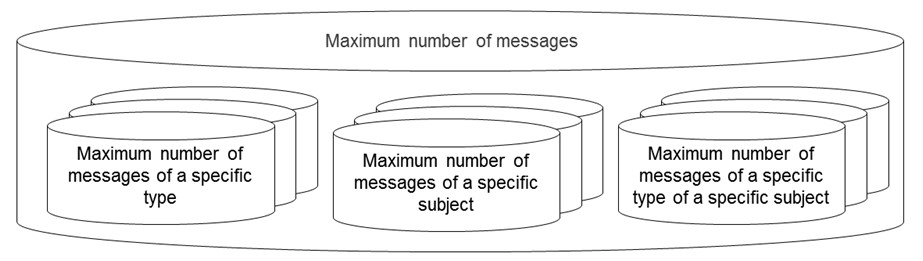
\includegraphics[width=12cm]{Figures/Ontology/SubjectInteraction/input-pool-informal.jpg}
	\caption[Input Pool]{Configuration of Input Pool Parameters}
	\label{fig:input-pool}
\end{figure*}

By restricting the size of the input pool, the ability of sending subjects to place messages in the input pool may be blocked at a certain point in time during process execution. If any value is set to zero this of course only allows for synchronous communication by default. However, if the the limit is higher than zero a run-time-environment must decide how to handle the input pool. There are four strategies to handle input in regards to a specific restriction that can be included into PASS.

\begin{itemize}
	\item \textbf{Blocking the sender} --- Once all slots are occupied in an input pool, the sender is blocked until the receiving subject picks up a message (i.e. a message is removed from the input pool). This creates space for a new message. In case several subjects want to put a message into a fully occupied input pool, the subject that has been waiting longest for an empty slot is allowed to send. The procedure is analogous if corresponding input pool parameters do not allow storing the message in the input pool, i.e., if the corresponding number of messages of the same name or from the same subject has been put into the input pool.
	\item \textbf{Delete the oldest message} --- In case all the slots are already occupied in the input pool of the subject addressed, the oldest message is overwritten with the new message.
	\item \textbf{Delete the latest message} --- The latest message is deleted from the input pool to allow depositing of the new incoming message. If all the positions in the input pool of the addressed subject are taken, the latest message in the input pool is overwritten with the new message. This strategy applies analogously when the maximum number of messages in the input pool has been reached, either concerning sender or message type.
	\item \textbf{Dropping the new message after reception} ---
\end{itemize}